\documentclass[1p]{elsarticle_modified}
%\bibliographystyle{elsarticle-num}

%\usepackage[colorlinks]{hyperref}
%\usepackage{abbrmath_seonhwa} %\Abb, \Ascr, \Acal ,\Abf, \Afrak
\usepackage{amsfonts}
\usepackage{amssymb}
\usepackage{amsmath}
\usepackage{amsthm}
\usepackage{scalefnt}
\usepackage{amsbsy}
\usepackage{kotex}
\usepackage{caption}
\usepackage{subfig}
\usepackage{color}
\usepackage{graphicx}
\usepackage{xcolor} %% white, black, red, green, blue, cyan, magenta, yellow
\usepackage{float}
\usepackage{setspace}
\usepackage{hyperref}

\usepackage{tikz}
\usetikzlibrary{arrows}

\usepackage{multirow}
\usepackage{array} % fixed length table
\usepackage{hhline}

%%%%%%%%%%%%%%%%%%%%%
\makeatletter
\renewcommand*\env@matrix[1][\arraystretch]{%
	\edef\arraystretch{#1}%
	\hskip -\arraycolsep
	\let\@ifnextchar\new@ifnextchar
	\array{*\c@MaxMatrixCols c}}
\makeatother %https://tex.stackexchange.com/questions/14071/how-can-i-increase-the-line-spacing-in-a-matrix
%%%%%%%%%%%%%%%

\usepackage[normalem]{ulem}

\newcommand{\msout}[1]{\ifmmode\text{\sout{\ensuremath{#1}}}\else\sout{#1}\fi}
%SOURCE: \msout is \stkout macro in https://tex.stackexchange.com/questions/20609/strikeout-in-math-mode

\newcommand{\cancel}[1]{
	\ifmmode
	{\color{red}\msout{#1}}
	\else
	{\color{red}\sout{#1}}
	\fi
}

\newcommand{\add}[1]{
	{\color{blue}\uwave{#1}}
}

\newcommand{\replace}[2]{
	\ifmmode
	{\color{red}\msout{#1}}{\color{blue}\uwave{#2}}
	\else
	{\color{red}\sout{#1}}{\color{blue}\uwave{#2}}
	\fi
}

\newcommand{\Sol}{\mathcal{S}} %segment
\newcommand{\D}{D} %diagram
\newcommand{\A}{\mathcal{A}} %arc


%%%%%%%%%%%%%%%%%%%%%%%%%%%%%5 test

\def\sl{\operatorname{\textup{SL}}(2,\Cbb)}
\def\psl{\operatorname{\textup{PSL}}(2,\Cbb)}
\def\quan{\mkern 1mu \triangleright \mkern 1mu}

\theoremstyle{definition}
\newtheorem{thm}{Theorem}[section]
\newtheorem{prop}[thm]{Proposition}
\newtheorem{lem}[thm]{Lemma}
\newtheorem{ques}[thm]{Question}
\newtheorem{cor}[thm]{Corollary}
\newtheorem{defn}[thm]{Definition}
\newtheorem{exam}[thm]{Example}
\newtheorem{rmk}[thm]{Remark}
\newtheorem{alg}[thm]{Algorithm}

\newcommand{\I}{\sqrt{-1}}
\begin{document}

%\begin{frontmatter}
%
%\title{Boundary parabolic representations of knots up to 8 crossings}
%
%%% Group authors per affiliation:
%\author{Yunhi Cho} 
%\address{Department of Mathematics, University of Seoul, Seoul, Korea}
%\ead{yhcho@uos.ac.kr}
%
%
%\author{Seonhwa Kim} %\fnref{s_kim}}
%\address{Center for Geometry and Physics, Institute for Basic Science, Pohang, 37673, Korea}
%\ead{ryeona17@ibs.re.kr}
%
%\author{Hyuk Kim}
%\address{Department of Mathematical Sciences, Seoul National University, Seoul 08826, Korea}
%\ead{hyukkim@snu.ac.kr}
%
%\author{Seokbeom Yoon}
%\address{Department of Mathematical Sciences, Seoul National University, Seoul, 08826,  Korea}
%\ead{sbyoon15@snu.ac.kr}
%
%\begin{abstract}
%We find all boundary parabolic representation of knots up to 8 crossings.
%
%\end{abstract}
%\begin{keyword}
%    \MSC[2010] 57M25 
%\end{keyword}
%
%\end{frontmatter}

%\linenumbers
%\tableofcontents
%
\newcommand\colored[1]{\textcolor{white}{\rule[-0.35ex]{0.8em}{1.4ex}}\kern-0.8em\color{red} #1}%
%\newcommand\colored[1]{\textcolor{white}{ #1}\kern-2.17ex	\textcolor{white}{ #1}\kern-1.81ex	\textcolor{white}{ #1}\kern-2.15ex\color{red}#1	}

{\Large $\underline{12a_{0686}~(K12a_{0686})}$}

\setlength{\tabcolsep}{10pt}
\renewcommand{\arraystretch}{1.6}
\vspace{1cm}\begin{tabular}{m{100pt}>{\centering\arraybackslash}m{274pt}}
\multirow{5}{120pt}{
	\centering
	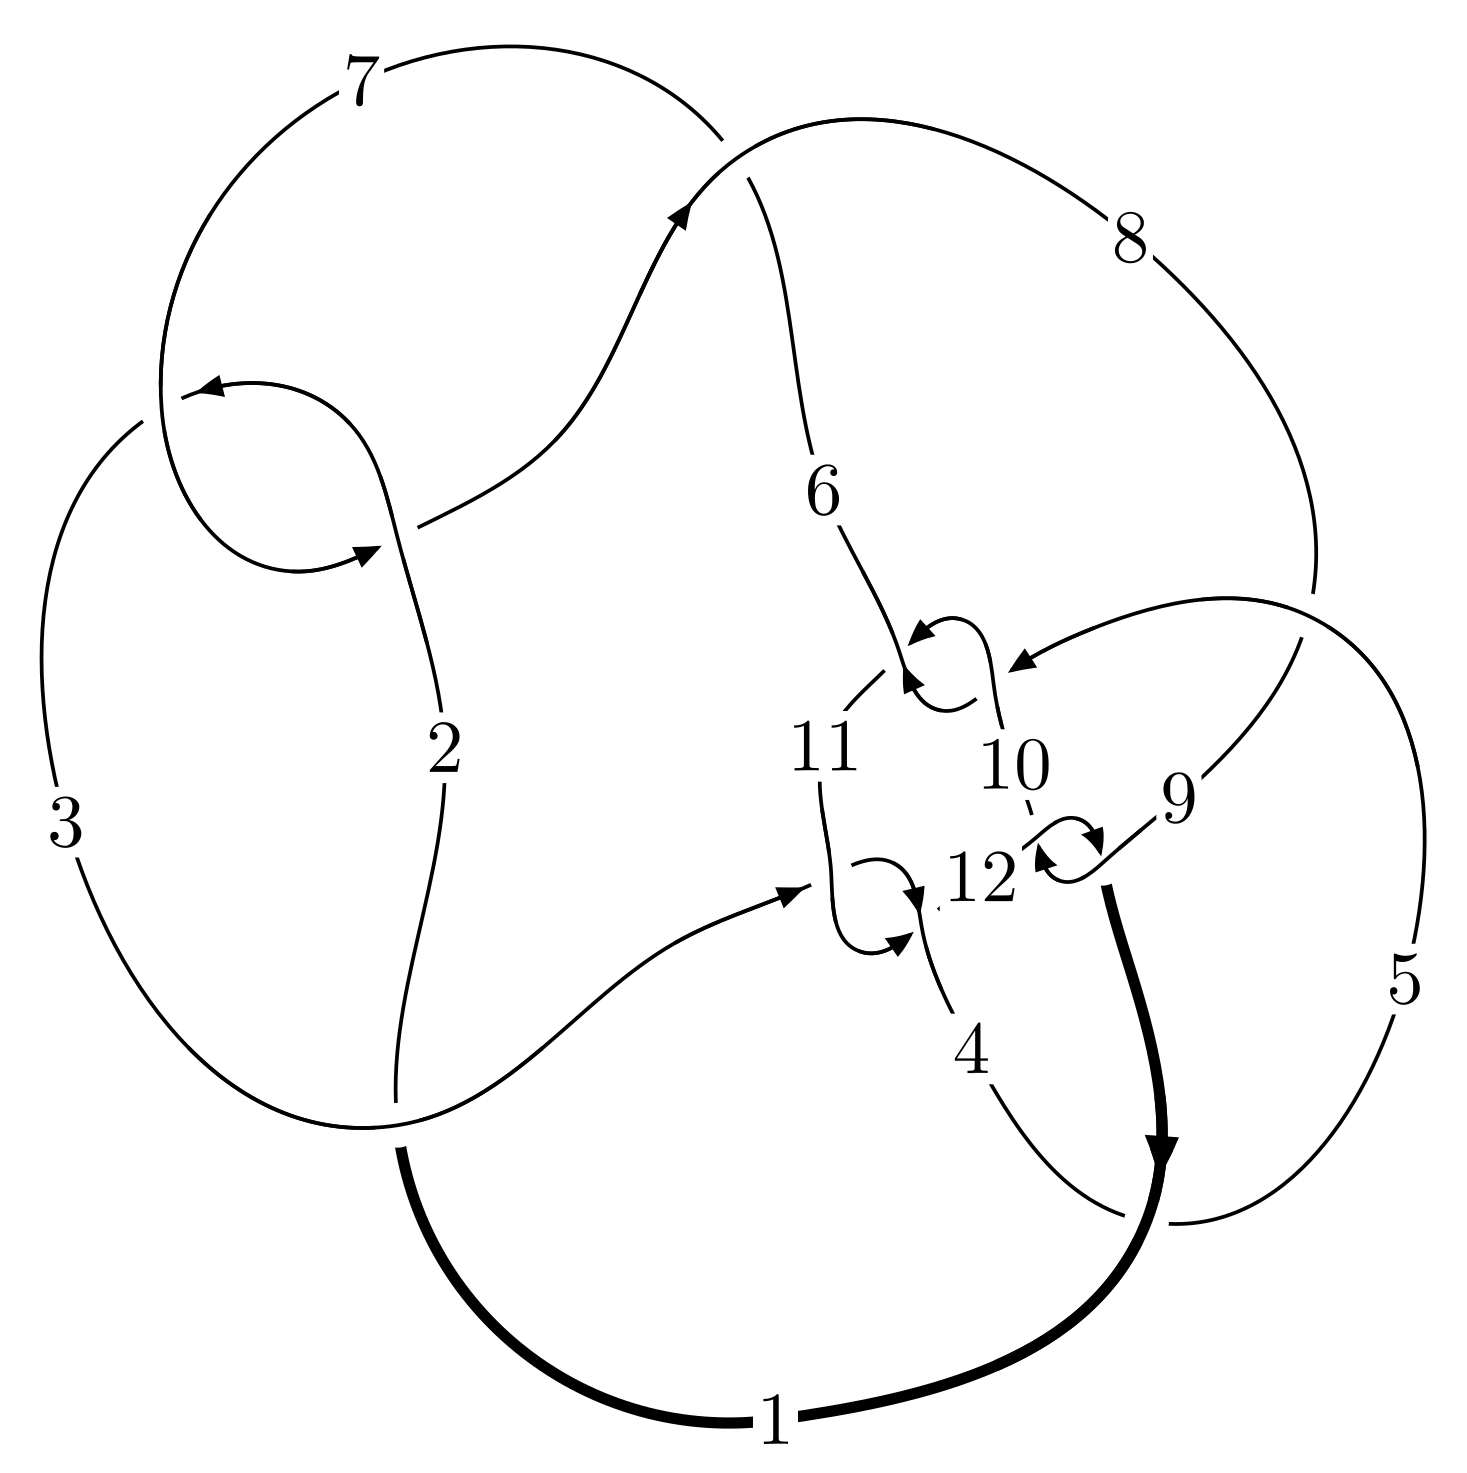
\includegraphics[width=112pt]{../../../GIT/diagram.site/Diagrams/png/1487_12a_0686.png}\\
\ \ \ A knot diagram\footnotemark}&
\allowdisplaybreaks
\textbf{Linearized knot diagam} \\
\cline{2-2}
 &
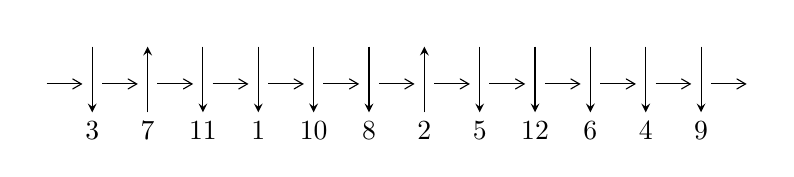
\begin{tikzpicture}[x=20pt, y=17pt]
	% nodes
	\node (C0) at (0, 0) {};
	\node (C1) at (1, 0) {};
	\node (C1U) at (1, +1) {};
	\node (C1D) at (1, -1) {3};

	\node (C2) at (2, 0) {};
	\node (C2U) at (2, +1) {};
	\node (C2D) at (2, -1) {7};

	\node (C3) at (3, 0) {};
	\node (C3U) at (3, +1) {};
	\node (C3D) at (3, -1) {11};

	\node (C4) at (4, 0) {};
	\node (C4U) at (4, +1) {};
	\node (C4D) at (4, -1) {1};

	\node (C5) at (5, 0) {};
	\node (C5U) at (5, +1) {};
	\node (C5D) at (5, -1) {10};

	\node (C6) at (6, 0) {};
	\node (C6U) at (6, +1) {};
	\node (C6D) at (6, -1) {8};

	\node (C7) at (7, 0) {};
	\node (C7U) at (7, +1) {};
	\node (C7D) at (7, -1) {2};

	\node (C8) at (8, 0) {};
	\node (C8U) at (8, +1) {};
	\node (C8D) at (8, -1) {5};

	\node (C9) at (9, 0) {};
	\node (C9U) at (9, +1) {};
	\node (C9D) at (9, -1) {12};

	\node (C10) at (10, 0) {};
	\node (C10U) at (10, +1) {};
	\node (C10D) at (10, -1) {6};

	\node (C11) at (11, 0) {};
	\node (C11U) at (11, +1) {};
	\node (C11D) at (11, -1) {4};

	\node (C12) at (12, 0) {};
	\node (C12U) at (12, +1) {};
	\node (C12D) at (12, -1) {9};
	\node (C13) at (13, 0) {};

	% arrows
	\draw[->,>={angle 60}]
	(C0) edge (C1) (C1) edge (C2) (C2) edge (C3) (C3) edge (C4) (C4) edge (C5) (C5) edge (C6) (C6) edge (C7) (C7) edge (C8) (C8) edge (C9) (C9) edge (C10) (C10) edge (C11) (C11) edge (C12) (C12) edge (C13) ;	\draw[->,>=stealth]
	(C1U) edge (C1D) (C2D) edge (C2U) (C3U) edge (C3D) (C4U) edge (C4D) (C5U) edge (C5D) (C6U) edge (C6D) (C7D) edge (C7U) (C8U) edge (C8D) (C9U) edge (C9D) (C10U) edge (C10D) (C11U) edge (C11D) (C12U) edge (C12D) ;
	\end{tikzpicture} \\
\hhline{~~} \\& 
\textbf{Solving Sequence} \\ \cline{2-2} 
 &
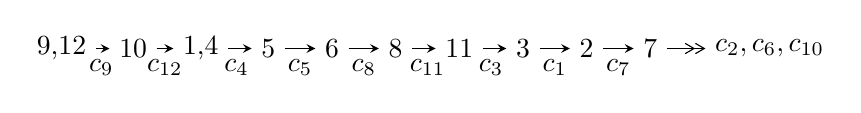
\begin{tikzpicture}[x=23pt, y=7pt]
	% node
	\node (A0) at (-1/8, 0) {9,12};
	\node (A1) at (1, 0) {10};
	\node (A2) at (33/16, 0) {1,4};
	\node (A3) at (25/8, 0) {5};
	\node (A4) at (33/8, 0) {6};
	\node (A5) at (41/8, 0) {8};
	\node (A6) at (49/8, 0) {11};
	\node (A7) at (57/8, 0) {3};
	\node (A8) at (65/8, 0) {2};
	\node (A9) at (73/8, 0) {7};
	\node (C1) at (1/2, -1) {$c_{9}$};
	\node (C2) at (3/2, -1) {$c_{12}$};
	\node (C3) at (21/8, -1) {$c_{4}$};
	\node (C4) at (29/8, -1) {$c_{5}$};
	\node (C5) at (37/8, -1) {$c_{8}$};
	\node (C6) at (45/8, -1) {$c_{11}$};
	\node (C7) at (53/8, -1) {$c_{3}$};
	\node (C8) at (61/8, -1) {$c_{1}$};
	\node (C9) at (69/8, -1) {$c_{7}$};
	\node (A10) at (11, 0) {$c_{2},c_{6},c_{10}$};

	% edge
	\draw[->,>=stealth]	
	(A0) edge (A1) (A1) edge (A2) (A2) edge (A3) (A3) edge (A4) (A4) edge (A5) (A5) edge (A6) (A6) edge (A7) (A7) edge (A8) (A8) edge (A9) ;
	\draw[->>,>={angle 60}]	
	(A9) edge (A10);
\end{tikzpicture} \\ 

\end{tabular} \\

\footnotetext{
The image of knot diagram is generated by the software ``\textbf{Draw programme}" developed by Andrew Bartholomew(\url{http://www.layer8.co.uk/maths/draw/index.htm\#Running-draw}), where we modified some parts for our purpose(\url{https://github.com/CATsTAILs/LinksPainter}).
}\phantom \\ \newline 
\centering \textbf{Ideals for irreducible components\footnotemark of $X_{\text{par}}$} 
 
\begin{align*}
I^u_{1}&=\langle 
-3587 u^{44}-59411 u^{43}+\cdots+256 b-2894080,\;-1823 u^{44}-49813 u^{43}+\cdots+512 a+5447424,\\
\phantom{I^u_{1}}&\phantom{= \langle  }u^{45}+21 u^{44}+\cdots-9728 u-512\rangle \\
I^u_{2}&=\langle 
-7.59604\times10^{31} a^{17} u^{4}-1.14352\times10^{32} a^{16} u^{4}+\cdots+1.79108\times10^{32} a-3.77085\times10^{32},\\
\phantom{I^u_{2}}&\phantom{= \langle  }-6 a^{16} u^4+a^{15} u^4+\cdots-180 a+371,\;u^5- u^4+2 u^3- u^2+u-1\rangle \\
I^u_{3}&=\langle 
-27 u^{30}+186 u^{29}+\cdots+b+53,\;-29 u^{30}+147 u^{29}+\cdots+a-64,\;u^{31}-6 u^{30}+\cdots+5 u^2+1\rangle \\
\\
\end{align*}
\raggedright * 3 irreducible components of $\dim_{\mathbb{C}}=0$, with total 166 representations.\\
\footnotetext{All coefficients of polynomials are rational numbers. But the coefficients are sometimes approximated in decimal forms when there is not enough margin.}
\newpage
\renewcommand{\arraystretch}{1}
\centering \section*{I. $I^u_{1}= \langle -3587 u^{44}-59411 u^{43}+\cdots+256 b-2894080,\;-1823 u^{44}-49813 u^{43}+\cdots+512 a+5447424,\;u^{45}+21 u^{44}+\cdots-9728 u-512 \rangle$}
\flushleft \textbf{(i) Arc colorings}\\
\begin{tabular}{m{7pt} m{180pt} m{7pt} m{180pt} }
\flushright $a_{9}=$&$\begin{pmatrix}1\\0\end{pmatrix}$ \\
\flushright $a_{12}=$&$\begin{pmatrix}0\\u\end{pmatrix}$ \\
\flushright $a_{10}=$&$\begin{pmatrix}1\\u^2\end{pmatrix}$ \\
\flushright $a_{1}=$&$\begin{pmatrix}- u\\u\end{pmatrix}$ \\
\flushright $a_{4}=$&$\begin{pmatrix}3.56055 u^{44}+97.2910 u^{43}+\cdots-191511. u-10639.5\\14.0117 u^{44}+232.074 u^{43}+\cdots+205133. u+11305\end{pmatrix}$ \\
\flushright $a_{5}=$&$\begin{pmatrix}-22.0801 u^{44}-477.693 u^{43}+\cdots+185231. u+9662.50\\39.6523 u^{44}+807.059 u^{43}+\cdots-171609. u-8997\end{pmatrix}$ \\
\flushright $a_{6}=$&$\begin{pmatrix}0.439453 u^{44}-28.7363 u^{43}+\cdots+209228 u+11485.5\\15.2461 u^{44}+383.090 u^{43}+\cdots-393095. u-21261\end{pmatrix}$ \\
\flushright $a_{8}=$&$\begin{pmatrix}-\frac{529}{512} u^{44}-\frac{10591}{512} u^{43}+\cdots+\frac{1243}{2} u+7\\\frac{135}{256} u^{44}+\frac{2441}{256} u^{43}+\cdots+4656 u+259\end{pmatrix}$ \\
\flushright $a_{11}=$&$\begin{pmatrix}\frac{253}{512} u^{44}+\frac{5043}{512} u^{43}+\cdots-\frac{8899}{2} u-247\\\frac{3}{256} u^{44}+\frac{77}{256} u^{43}+\cdots-317 u-17\end{pmatrix}$ \\
\flushright $a_{3}=$&$\begin{pmatrix}44.9453 u^{44}+910.176 u^{43}+\cdots-198900. u-10595.5\\-56.2461 u^{44}-1117.62 u^{43}+\cdots+82288.5 u+3722\end{pmatrix}$ \\
\flushright $a_{2}=$&$\begin{pmatrix}-4.48047 u^{44}-89.4336 u^{43}+\cdots+34007 u+1918\\\frac{129}{32} u^{44}+\frac{10127}{128} u^{43}+\cdots-4053 u-180\end{pmatrix}$ \\
\flushright $a_{7}=$&$\begin{pmatrix}-50.0195 u^{44}-1013.30 u^{43}+\cdots+228759. u+12212\\60.0117 u^{44}+1189.50 u^{43}+\cdots-71845 u-3052\end{pmatrix}$\\&\end{tabular}
\flushleft \textbf{(ii) Obstruction class $= -1$}\\~\\
\flushleft \textbf{(iii) Cusp Shapes $= \frac{679}{64} u^{44}+\frac{17161}{64} u^{43}+\cdots-240458 u-12510$}\\~\\
\newpage\renewcommand{\arraystretch}{1}
\flushleft \textbf{(iv) u-Polynomials at the component}\newline \\
\begin{tabular}{m{50pt}|m{274pt}}
Crossings & \hspace{64pt}u-Polynomials at each crossing \\
\hline $$\begin{aligned}c_{1},c_{6}\end{aligned}$$&$\begin{aligned}
&u^{45}+15 u^{44}+\cdots-1536 u-1024
\end{aligned}$\\
\hline $$\begin{aligned}c_{2},c_{7}\end{aligned}$$&$\begin{aligned}
&u^{45}+11 u^{44}+\cdots+128 u+32
\end{aligned}$\\
\hline $$\begin{aligned}c_{3},c_{5},c_{10}\\c_{11}\end{aligned}$$&$\begin{aligned}
&u^{45}+u^{44}+\cdots+4 u+1
\end{aligned}$\\
\hline $$\begin{aligned}c_{4},c_{8}\end{aligned}$$&$\begin{aligned}
&u^{45}- u^{44}+\cdots-5 u+1
\end{aligned}$\\
\hline $$\begin{aligned}c_{9},c_{12}\end{aligned}$$&$\begin{aligned}
&u^{45}-21 u^{44}+\cdots-9728 u+512
\end{aligned}$\\
\hline
\end{tabular}\\~\\
\newpage\renewcommand{\arraystretch}{1}
\flushleft \textbf{(v) Riley Polynomials at the component}\newline \\
\begin{tabular}{m{50pt}|m{274pt}}
Crossings & \hspace{64pt}Riley Polynomials at each crossing \\
\hline $$\begin{aligned}c_{1},c_{6}\end{aligned}$$&$\begin{aligned}
&y^{45}+31 y^{44}+\cdots+9830400 y-1048576
\end{aligned}$\\
\hline $$\begin{aligned}c_{2},c_{7}\end{aligned}$$&$\begin{aligned}
&y^{45}+15 y^{44}+\cdots-1536 y-1024
\end{aligned}$\\
\hline $$\begin{aligned}c_{3},c_{5},c_{10}\\c_{11}\end{aligned}$$&$\begin{aligned}
&y^{45}-25 y^{44}+\cdots+8 y-1
\end{aligned}$\\
\hline $$\begin{aligned}c_{4},c_{8}\end{aligned}$$&$\begin{aligned}
&y^{45}+29 y^{44}+\cdots+71 y-1
\end{aligned}$\\
\hline $$\begin{aligned}c_{9},c_{12}\end{aligned}$$&$\begin{aligned}
&y^{45}+17 y^{44}+\cdots-3407872 y-262144
\end{aligned}$\\
\hline
\end{tabular}\\~\\
\newpage\flushleft \textbf{(vi) Complex Volumes and Cusp Shapes}
$$\begin{array}{c|c|c}  
\text{Solutions to }I^u_{1}& \I (\text{vol} + \sqrt{-1}CS) & \text{Cusp shape}\\
 \hline 
\begin{aligned}
u &= -0.208020 + 1.017770 I \\
a &= \phantom{-}0.518836 - 0.448183 I \\
b &= -1.46031 - 0.10701 I\end{aligned}
 & \phantom{-}1.31767 + 2.83862 I & \phantom{-0.000000 } 0 \\ \hline\begin{aligned}
u &= -0.208020 - 1.017770 I \\
a &= \phantom{-}0.518836 + 0.448183 I \\
b &= -1.46031 + 0.10701 I\end{aligned}
 & \phantom{-}1.31767 - 2.83862 I & \phantom{-0.000000 } 0 \\ \hline\begin{aligned}
u &= \phantom{-}0.946189\phantom{ +0.000000I} \\
a &= \phantom{-}0.633784\phantom{ +0.000000I} \\
b &= -0.410735\phantom{ +0.000000I}\end{aligned}
 & -1.39480\phantom{ +0.000000I} & \phantom{-0.000000 } 0 \\ \hline\begin{aligned}
u &= -1.063240 + 0.314250 I \\
a &= -0.886556 - 0.815280 I \\
b &= \phantom{-}0.350469 - 0.222476 I\end{aligned}
 & -0.95255 - 6.81200 I & \phantom{-0.000000 } 0 \\ \hline\begin{aligned}
u &= -1.063240 - 0.314250 I \\
a &= -0.886556 + 0.815280 I \\
b &= \phantom{-}0.350469 + 0.222476 I\end{aligned}
 & -0.95255 + 6.81200 I & \phantom{-0.000000 } 0 \\ \hline\begin{aligned}
u &= -1.079690 + 0.283438 I \\
a &= \phantom{-}0.962572 + 0.810776 I \\
b &= -0.335797 + 0.200198 I\end{aligned}
 & -2.25231 - 12.86870 I & \phantom{-0.000000 } 0 \\ \hline\begin{aligned}
u &= -1.079690 - 0.283438 I \\
a &= \phantom{-}0.962572 - 0.810776 I \\
b &= -0.335797 - 0.200198 I\end{aligned}
 & -2.25231 + 12.86870 I & \phantom{-0.000000 } 0 \\ \hline\begin{aligned}
u &= -0.143066 + 1.150190 I \\
a &= -0.542252 + 0.522617 I \\
b &= \phantom{-}1.310810 - 0.279245 I\end{aligned}
 & \phantom{-}3.41317 - 0.45131 I & \phantom{-0.000000 } 0 \\ \hline\begin{aligned}
u &= -0.143066 - 1.150190 I \\
a &= -0.542252 - 0.522617 I \\
b &= \phantom{-}1.310810 + 0.279245 I\end{aligned}
 & \phantom{-}3.41317 + 0.45131 I & \phantom{-0.000000 } 0 \\ \hline\begin{aligned}
u &= -0.336154 + 1.112550 I \\
a &= \phantom{-}0.676007 - 0.377814 I \\
b &= -1.97704 + 0.16844 I\end{aligned}
 & \phantom{-}8.08821 + 6.31292 I & \phantom{-0.000000 } 0\\
 \hline 
 \end{array}$$\newpage$$\begin{array}{c|c|c}  
\text{Solutions to }I^u_{1}& \I (\text{vol} + \sqrt{-1}CS) & \text{Cusp shape}\\
 \hline 
\begin{aligned}
u &= -0.336154 - 1.112550 I \\
a &= \phantom{-}0.676007 + 0.377814 I \\
b &= -1.97704 - 0.16844 I\end{aligned}
 & \phantom{-}8.08821 - 6.31292 I & \phantom{-0.000000 } 0 \\ \hline\begin{aligned}
u &= -0.317978 + 1.137660 I \\
a &= -0.686649 + 0.428740 I \\
b &= \phantom{-}1.90789 - 0.27801 I\end{aligned}
 & \phantom{-}8.41961 + 0.29227 I & \phantom{-0.000000 } 0 \\ \hline\begin{aligned}
u &= -0.317978 - 1.137660 I \\
a &= -0.686649 - 0.428740 I \\
b &= \phantom{-}1.90789 + 0.27801 I\end{aligned}
 & \phantom{-}8.41961 - 0.29227 I & \phantom{-0.000000 } 0 \\ \hline\begin{aligned}
u &= -1.094150 + 0.527804 I \\
a &= -0.656726 - 0.627002 I \\
b &= \phantom{-}0.518635 - 0.238568 I\end{aligned}
 & -3.21307 - 2.60752 I & \phantom{-0.000000 } 0 \\ \hline\begin{aligned}
u &= -1.094150 - 0.527804 I \\
a &= -0.656726 + 0.627002 I \\
b &= \phantom{-}0.518635 + 0.238568 I\end{aligned}
 & -3.21307 + 2.60752 I & \phantom{-0.000000 } 0 \\ \hline\begin{aligned}
u &= -0.766388 + 0.963185 I \\
a &= -0.482755 - 0.428981 I \\
b &= \phantom{-}1.47163 - 0.30603 I\end{aligned}
 & \phantom{-}5.84298 - 0.38109 I & \phantom{-0.000000 } 0 \\ \hline\begin{aligned}
u &= -0.766388 - 0.963185 I \\
a &= -0.482755 + 0.428981 I \\
b &= \phantom{-}1.47163 + 0.30603 I\end{aligned}
 & \phantom{-}5.84298 + 0.38109 I & \phantom{-0.000000 } 0 \\ \hline\begin{aligned}
u &= -1.174520 + 0.378645 I \\
a &= \phantom{-}0.843485 + 0.605476 I \\
b &= -0.421155 + 0.168073 I\end{aligned}
 & -8.33701 - 5.85390 I & \phantom{-0.000000 } 0 \\ \hline\begin{aligned}
u &= -1.174520 - 0.378645 I \\
a &= \phantom{-}0.843485 - 0.605476 I \\
b &= -0.421155 - 0.168073 I\end{aligned}
 & -8.33701 + 5.85390 I & \phantom{-0.000000 } 0 \\ \hline\begin{aligned}
u &= -0.736297 + 1.018030 I \\
a &= \phantom{-}0.528992 + 0.406341 I \\
b &= -1.64434 + 0.15871 I\end{aligned}
 & \phantom{-}6.06401 + 6.26641 I & \phantom{-0.000000 } 0\\
 \hline 
 \end{array}$$\newpage$$\begin{array}{c|c|c}  
\text{Solutions to }I^u_{1}& \I (\text{vol} + \sqrt{-1}CS) & \text{Cusp shape}\\
 \hline 
\begin{aligned}
u &= -0.736297 - 1.018030 I \\
a &= \phantom{-}0.528992 - 0.406341 I \\
b &= -1.64434 - 0.15871 I\end{aligned}
 & \phantom{-}6.06401 - 6.26641 I & \phantom{-0.000000 } 0 \\ \hline\begin{aligned}
u &= \phantom{-}0.133405 + 1.254510 I \\
a &= \phantom{-}0.447547 - 0.505637 I \\
b &= -0.814640 + 0.321639 I\end{aligned}
 & -0.52886 - 2.12424 I & \phantom{-0.000000 } 0 \\ \hline\begin{aligned}
u &= \phantom{-}0.133405 - 1.254510 I \\
a &= \phantom{-}0.447547 + 0.505637 I \\
b &= -0.814640 - 0.321639 I\end{aligned}
 & -0.52886 + 2.12424 I & \phantom{-0.000000 } 0 \\ \hline\begin{aligned}
u &= -0.138187 + 1.365490 I \\
a &= -0.470658 + 0.644285 I \\
b &= \phantom{-}1.036310 - 0.731066 I\end{aligned}
 & \phantom{-}5.34883 - 2.70325 I & \phantom{-0.000000 } 0 \\ \hline\begin{aligned}
u &= -0.138187 - 1.365490 I \\
a &= -0.470658 - 0.644285 I \\
b &= \phantom{-}1.036310 + 0.731066 I\end{aligned}
 & \phantom{-}5.34883 + 2.70325 I & \phantom{-0.000000 } 0 \\ \hline\begin{aligned}
u &= -1.206150 + 0.670708 I \\
a &= \phantom{-}0.608172 + 0.509443 I \\
b &= -0.606059 + 0.130819 I\end{aligned}
 & -6.10066 + 2.59329 I & \phantom{-0.000000 } 0 \\ \hline\begin{aligned}
u &= -1.206150 - 0.670708 I \\
a &= \phantom{-}0.608172 - 0.509443 I \\
b &= -0.606059 - 0.130819 I\end{aligned}
 & -6.10066 - 2.59329 I & \phantom{-0.000000 } 0 \\ \hline\begin{aligned}
u &= -0.635659 + 1.245840 I \\
a &= \phantom{-}0.886702 + 0.620717 I \\
b &= -2.12868 - 0.87707 I\end{aligned}
 & \phantom{-}1.98718 + 12.88950 I & \phantom{-0.000000 } 0 \\ \hline\begin{aligned}
u &= -0.635659 - 1.245840 I \\
a &= \phantom{-}0.886702 - 0.620717 I \\
b &= -2.12868 + 0.87707 I\end{aligned}
 & \phantom{-}1.98718 - 12.88950 I & \phantom{-0.000000 } 0 \\ \hline\begin{aligned}
u &= -0.694335 + 1.218240 I \\
a &= \phantom{-}0.726779 + 0.567265 I \\
b &= -1.81930 - 0.63902 I\end{aligned}
 & -0.87266 + 9.07868 I & \phantom{-0.000000 } 0\\
 \hline 
 \end{array}$$\newpage$$\begin{array}{c|c|c}  
\text{Solutions to }I^u_{1}& \I (\text{vol} + \sqrt{-1}CS) & \text{Cusp shape}\\
 \hline 
\begin{aligned}
u &= -0.694335 - 1.218240 I \\
a &= \phantom{-}0.726779 - 0.567265 I \\
b &= -1.81930 + 0.63902 I\end{aligned}
 & -0.87266 - 9.07868 I & \phantom{-0.000000 } 0 \\ \hline\begin{aligned}
u &= -0.631447 + 1.256290 I \\
a &= -0.904289 - 0.657496 I \\
b &= \phantom{-}2.14391 + 0.96340 I\end{aligned}
 & \phantom{-}0.8069 + 18.9599 I & \phantom{-0.000000 } 0 \\ \hline\begin{aligned}
u &= -0.631447 - 1.256290 I \\
a &= -0.904289 + 0.657496 I \\
b &= \phantom{-}2.14391 - 0.96340 I\end{aligned}
 & \phantom{-}0.8069 - 18.9599 I & \phantom{-0.000000 } 0 \\ \hline\begin{aligned}
u &= -0.587391 + 0.037334 I \\
a &= -0.021046 - 1.328720 I \\
b &= \phantom{-}0.008378 - 0.428391 I\end{aligned}
 & \phantom{-}5.05448 - 2.94618 I & -3.07738 + 3.17176 I \\ \hline\begin{aligned}
u &= -0.587391 - 0.037334 I \\
a &= -0.021046 + 1.328720 I \\
b &= \phantom{-}0.008378 + 0.428391 I\end{aligned}
 & \phantom{-}5.05448 + 2.94618 I & -3.07738 - 3.17176 I \\ \hline\begin{aligned}
u &= -0.67285 + 1.26135 I \\
a &= -0.773811 - 0.664467 I \\
b &= \phantom{-}1.85557 + 0.90212 I\end{aligned}
 & -5.45040 + 12.36210 I & \phantom{-0.000000 } 0 \\ \hline\begin{aligned}
u &= -0.67285 - 1.26135 I \\
a &= -0.773811 + 0.664467 I \\
b &= \phantom{-}1.85557 - 0.90212 I\end{aligned}
 & -5.45040 - 12.36210 I & \phantom{-0.000000 } 0 \\ \hline\begin{aligned}
u &= -0.13532 + 1.43665 I \\
a &= \phantom{-}0.416738 - 0.663296 I \\
b &= -0.893009 + 0.802371 I\end{aligned}
 & \phantom{-}4.09263 - 8.37531 I & \phantom{-0.000000 } 0 \\ \hline\begin{aligned}
u &= -0.13532 - 1.43665 I \\
a &= \phantom{-}0.416738 + 0.663296 I \\
b &= -0.893009 - 0.802371 I\end{aligned}
 & \phantom{-}4.09263 + 8.37531 I & \phantom{-0.000000 } 0 \\ \hline\begin{aligned}
u &= -0.75657 + 1.23255 I \\
a &= -0.628948 - 0.591286 I \\
b &= \phantom{-}1.54134 + 0.61150 I\end{aligned}
 & -4.00755 + 4.49447 I & \phantom{-0.000000 } 0\\
 \hline 
 \end{array}$$\newpage$$\begin{array}{c|c|c}  
\text{Solutions to }I^u_{1}& \I (\text{vol} + \sqrt{-1}CS) & \text{Cusp shape}\\
 \hline 
\begin{aligned}
u &= -0.75657 - 1.23255 I \\
a &= -0.628948 + 0.591286 I \\
b &= \phantom{-}1.54134 - 0.61150 I\end{aligned}
 & -4.00755 - 4.49447 I & \phantom{-0.000000 } 0 \\ \hline\begin{aligned}
u &= \phantom{-}1.40518 + 0.43144 I \\
a &= -0.469825 + 0.097281 I \\
b &= \phantom{-}0.380597 - 0.039104 I\end{aligned}
 & -4.48294 - 3.96522 I & \phantom{-0.000000 } 0 \\ \hline\begin{aligned}
u &= \phantom{-}1.40518 - 0.43144 I \\
a &= -0.469825 - 0.097281 I \\
b &= \phantom{-}0.380597 + 0.039104 I\end{aligned}
 & -4.48294 + 3.96522 I & \phantom{-0.000000 } 0 \\ \hline\begin{aligned}
u &= -0.134253 + 0.255202 I \\
a &= \phantom{-}0.590793 - 1.189790 I \\
b &= -0.219829 - 0.348173 I\end{aligned}
 & -0.380823 - 0.987902 I & -6.30490 + 6.80539 I \\ \hline\begin{aligned}
u &= -0.134253 - 0.255202 I \\
a &= \phantom{-}0.590793 + 1.189790 I \\
b &= -0.219829 + 0.348173 I\end{aligned}
 & -0.380823 + 0.987902 I & -6.30490 - 6.80539 I\\
 \hline 
 \end{array}$$\newpage\newpage\renewcommand{\arraystretch}{1}
\centering \section*{II. $I^u_{2}= \langle -7.60\times10^{31} a^{17} u^{4}-1.14\times10^{32} a^{16} u^{4}+\cdots+1.79\times10^{32} a-3.77\times10^{32},\;-6 a^{16} u^4+a^{15} u^4+\cdots-180 a+371,\;u^5- u^4+2 u^3- u^2+u-1 \rangle$}
\flushleft \textbf{(i) Arc colorings}\\
\begin{tabular}{m{7pt} m{180pt} m{7pt} m{180pt} }
\flushright $a_{9}=$&$\begin{pmatrix}1\\0\end{pmatrix}$ \\
\flushright $a_{12}=$&$\begin{pmatrix}0\\u\end{pmatrix}$ \\
\flushright $a_{10}=$&$\begin{pmatrix}1\\u^2\end{pmatrix}$ \\
\flushright $a_{1}=$&$\begin{pmatrix}- u\\u\end{pmatrix}$ \\
\flushright $a_{4}=$&$\begin{pmatrix}a\\4.12624 a^{17} u^{4}+6.21168 a^{16} u^{4}+\cdots-9.72933 a+20.4836\end{pmatrix}$ \\
\flushright $a_{5}=$&$\begin{pmatrix}-4.60935 a^{17} u^{4}+9.84481 a^{16} u^{4}+\cdots+7.58983 a-12.3949\\8.73559 a^{17} u^{4}-3.63312 a^{16} u^{4}+\cdots-16.3192 a+32.8786\end{pmatrix}$ \\
\flushright $a_{6}=$&$\begin{pmatrix}9.19157 a^{17} u^{4}+6.07892 a^{16} u^{4}+\cdots+9.27627 a-17.7652\\-16.3897 a^{17} u^{4}-9.68706 a^{16} u^{4}+\cdots-11.3448 a+24.8604\end{pmatrix}$ \\
\flushright $a_{8}=$&$\begin{pmatrix}-0.209327 a^{17} u^{4}+8.30382 a^{16} u^{4}+\cdots-20.5251 a-19.9539\\7.76784 a^{17} u^{4}-5.15782 a^{16} u^{4}+\cdots+15.0521 a+8.28362\end{pmatrix}$ \\
\flushright $a_{11}=$&$\begin{pmatrix}a^2 u\\4.36914 a^{17} u^{4}+4.09814 a^{16} u^{4}+\cdots-37.3258 a-16.4733\end{pmatrix}$ \\
\flushright $a_{3}=$&$\begin{pmatrix}- a^3 u^2+a\\0.797957 a^{17} u^{4}+3.82143 a^{16} u^{4}+\cdots+6.45135 a-9.14231\end{pmatrix}$ \\
\flushright $a_{2}=$&$\begin{pmatrix}2.43152 a^{17} u^{4}-3.23675 a^{16} u^{4}+\cdots-6.46817 a+9.45064\\5.23364 a^{17} u^{4}+2.07480 a^{16} u^{4}+\cdots-22.9202 a-23.9576\end{pmatrix}$ \\
\flushright $a_{7}=$&$\begin{pmatrix}8.03403 a^{17} u^{4}+6.34108 a^{16} u^{4}+\cdots+13.2142 a-53.5432\\-11.0746 a^{17} u^{4}-5.17783 a^{16} u^{4}+\cdots-7.91911 a+18.8410\end{pmatrix}$\\&\end{tabular}
\flushleft \textbf{(ii) Obstruction class $= -1$}\\~\\
\flushleft \textbf{(iii) Cusp Shapes $= 2.46989 a^{17} u^{4}+15.4911 a^{16} u^{4}+\cdots-9.45003 a-119.435$}\\~\\
\newpage\renewcommand{\arraystretch}{1}
\flushleft \textbf{(iv) u-Polynomials at the component}\newline \\
\begin{tabular}{m{50pt}|m{274pt}}
Crossings & \hspace{64pt}u-Polynomials at each crossing \\
\hline $$\begin{aligned}c_{1},c_{6}\end{aligned}$$&$\begin{aligned}
&(u^9+3 u^8+8 u^7+13 u^6+17 u^5+17 u^4+12 u^3+6 u^2+u-1)^{10}
\end{aligned}$\\
\hline $$\begin{aligned}c_{2},c_{7}\end{aligned}$$&$\begin{aligned}
&(u^9- u^8+2 u^7- u^6+3 u^5- u^4+2 u^3+u+1)^{10}
\end{aligned}$\\
\hline $$\begin{aligned}c_{3},c_{5},c_{10}\\c_{11}\end{aligned}$$&$\begin{aligned}
&u^{90}+u^{89}+\cdots+651136 u+56443
\end{aligned}$\\
\hline $$\begin{aligned}c_{4},c_{8}\end{aligned}$$&$\begin{aligned}
&u^{90}-5 u^{89}+\cdots+14948 u-2189
\end{aligned}$\\
\hline $$\begin{aligned}c_{9},c_{12}\end{aligned}$$&$\begin{aligned}
&(u^5+u^4+2 u^3+u^2+u+1)^{18}
\end{aligned}$\\
\hline
\end{tabular}\\~\\
\newpage\renewcommand{\arraystretch}{1}
\flushleft \textbf{(v) Riley Polynomials at the component}\newline \\
\begin{tabular}{m{50pt}|m{274pt}}
Crossings & \hspace{64pt}Riley Polynomials at each crossing \\
\hline $$\begin{aligned}c_{1},c_{6}\end{aligned}$$&$\begin{aligned}
&(y^9+7 y^8+20 y^7+25 y^6+5 y^5-15 y^4+22 y^2+13 y-1)^{10}
\end{aligned}$\\
\hline $$\begin{aligned}c_{2},c_{7}\end{aligned}$$&$\begin{aligned}
&(y^9+3 y^8+8 y^7+13 y^6+17 y^5+17 y^4+12 y^3+6 y^2+y-1)^{10}
\end{aligned}$\\
\hline $$\begin{aligned}c_{3},c_{5},c_{10}\\c_{11}\end{aligned}$$&$\begin{aligned}
&y^{90}-65 y^{89}+\cdots-225222871104 y+3185812249
\end{aligned}$\\
\hline $$\begin{aligned}c_{4},c_{8}\end{aligned}$$&$\begin{aligned}
&y^{90}-13 y^{89}+\cdots-374991552 y+4791721
\end{aligned}$\\
\hline $$\begin{aligned}c_{9},c_{12}\end{aligned}$$&$\begin{aligned}
&(y^5+3 y^4+4 y^3+y^2- y-1)^{18}
\end{aligned}$\\
\hline
\end{tabular}\\~\\
\newpage\flushleft \textbf{(vi) Complex Volumes and Cusp Shapes}
$$\begin{array}{c|c|c}  
\text{Solutions to }I^u_{2}& \I (\text{vol} + \sqrt{-1}CS) & \text{Cusp shape}\\
 \hline 
\begin{aligned}
u &= -0.339110 + 0.822375 I \\
a &= -0.159381 - 0.938115 I \\
b &= \phantom{-}2.20160 + 1.42249 I\end{aligned}
 & -1.00758 - 5.55435 I & -9.90808 + 1.48270 I \\ \hline\begin{aligned}
u &= -0.339110 + 0.822375 I \\
a &= \phantom{-}0.241894 + 0.832836 I \\
b &= -2.08136 - 1.40087 I\end{aligned}
 & -0.234353 + 0.194409 I & -8.20079 - 3.72890 I \\ \hline\begin{aligned}
u &= -0.339110 + 0.822375 I \\
a &= -0.433799 - 1.204420 I \\
b &= \phantom{-}2.20036 + 1.00411 I\end{aligned}
 & -6.38914 - 0.56279 I & -15.9999 - 0.2678 I \\ \hline\begin{aligned}
u &= -0.339110 + 0.822375 I \\
a &= \phantom{-}0.826294 + 0.994064 I \\
b &= -1.83643 - 1.14645 I\end{aligned}
 & -3.40726 + 1.53058 I & -6.83254 - 4.43065 I \\ \hline\begin{aligned}
u &= -0.339110 + 0.822375 I \\
a &= -0.675713 - 1.117790 I \\
b &= \phantom{-}0.491959 - 1.241640 I\end{aligned}
 & -0.23435 + 2.86675 I & -8.20079 - 5.13240 I \\ \hline\begin{aligned}
u &= -0.339110 + 0.822375 I \\
a &= \phantom{-}0.763638 + 1.143180 I \\
b &= -0.68839 + 1.36569 I\end{aligned}
 & -1.00758 + 8.61551 I & -9.9081 - 10.3440 I \\ \hline\begin{aligned}
u &= -0.339110 + 0.822375 I \\
a &= -0.46396 - 1.45473 I \\
b &= \phantom{-}0.400574 - 0.166106 I\end{aligned}
 & -3.40726 + 1.53058 I & -6.83254 - 4.43065 I \\ \hline\begin{aligned}
u &= -0.339110 + 0.822375 I \\
a &= \phantom{-}1.40909 + 0.63481 I \\
b &= -1.91051 - 1.30463 I\end{aligned}
 & -0.23435 + 2.86675 I & -8.20079 - 5.13240 I \\ \hline\begin{aligned}
u &= -0.339110 + 0.822375 I \\
a &= \phantom{-}0.71153 + 1.38042 I \\
b &= -1.142030 + 0.739435 I\end{aligned}
 & -6.38914 + 3.62395 I & -15.9999 - 8.5935 I \\ \hline\begin{aligned}
u &= -0.339110 + 0.822375 I \\
a &= -0.59104 - 1.51012 I \\
b &= \phantom{-}2.18086 + 0.22940 I\end{aligned}
 & -3.98876 + 3.98500 I & -13.1570 - 7.3436 I\\
 \hline 
 \end{array}$$\newpage$$\begin{array}{c|c|c}  
\text{Solutions to }I^u_{2}& \I (\text{vol} + \sqrt{-1}CS) & \text{Cusp shape}\\
 \hline 
\begin{aligned}
u &= -0.339110 + 0.822375 I \\
a &= \phantom{-}0.05470 - 1.65936 I \\
b &= -0.581698 + 0.216015 I\end{aligned}
 & -0.234353 + 0.194409 I & -8.20079 - 3.72890 I \\ \hline\begin{aligned}
u &= -0.339110 + 0.822375 I \\
a &= \phantom{-}0.66566 + 1.53082 I \\
b &= -1.99721 + 0.11079 I\end{aligned}
 & -3.98876 - 0.92384 I & -13.15696 - 1.51767 I \\ \hline\begin{aligned}
u &= -0.339110 + 0.822375 I \\
a &= -1.55709 - 0.70875 I \\
b &= \phantom{-}1.93149 + 1.36749 I\end{aligned}
 & -1.00758 + 8.61551 I & -9.9081 - 10.3440 I \\ \hline\begin{aligned}
u &= -0.339110 + 0.822375 I \\
a &= -1.33525 - 1.17321 I \\
b &= \phantom{-}1.67468 + 1.37611 I\end{aligned}
 & -6.38914 + 3.62395 I & -15.9999 - 8.5935 I \\ \hline\begin{aligned}
u &= -0.339110 + 0.822375 I \\
a &= -0.07589 + 1.81158 I \\
b &= \phantom{-}0.631901 - 0.429114 I\end{aligned}
 & -1.00758 - 5.55435 I & -9.90808 + 1.48270 I \\ \hline\begin{aligned}
u &= -0.339110 + 0.822375 I \\
a &= \phantom{-}0.37937 + 1.85940 I \\
b &= -0.045624 - 0.663020 I\end{aligned}
 & -6.38914 - 0.56279 I & -15.9999 - 0.2678 I \\ \hline\begin{aligned}
u &= -0.339110 + 0.822375 I \\
a &= -1.14028 - 1.77640 I \\
b &= \phantom{-}1.06771 + 1.39994 I\end{aligned}
 & -3.98876 - 0.92384 I & -13.15696 - 1.51767 I \\ \hline\begin{aligned}
u &= -0.339110 + 0.822375 I \\
a &= \phantom{-}0.94152 + 1.91352 I \\
b &= -0.75943 - 1.29044 I\end{aligned}
 & -3.98876 + 3.98500 I & -13.1570 - 7.3436 I \\ \hline\begin{aligned}
u &= -0.339110 - 0.822375 I \\
a &= -0.159381 + 0.938115 I \\
b &= \phantom{-}2.20160 - 1.42249 I\end{aligned}
 & -1.00758 + 5.55435 I & -9.90808 - 1.48270 I \\ \hline\begin{aligned}
u &= -0.339110 - 0.822375 I \\
a &= \phantom{-}0.241894 - 0.832836 I \\
b &= -2.08136 + 1.40087 I\end{aligned}
 & -0.234353 - 0.194409 I & -8.20079 + 3.72890 I\\
 \hline 
 \end{array}$$\newpage$$\begin{array}{c|c|c}  
\text{Solutions to }I^u_{2}& \I (\text{vol} + \sqrt{-1}CS) & \text{Cusp shape}\\
 \hline 
\begin{aligned}
u &= -0.339110 - 0.822375 I \\
a &= -0.433799 + 1.204420 I \\
b &= \phantom{-}2.20036 - 1.00411 I\end{aligned}
 & -6.38914 + 0.56279 I & -15.9999 + 0.2678 I \\ \hline\begin{aligned}
u &= -0.339110 - 0.822375 I \\
a &= \phantom{-}0.826294 - 0.994064 I \\
b &= -1.83643 + 1.14645 I\end{aligned}
 & -3.40726 - 1.53058 I & -6.83254 + 4.43065 I \\ \hline\begin{aligned}
u &= -0.339110 - 0.822375 I \\
a &= -0.675713 + 1.117790 I \\
b &= \phantom{-}0.491959 + 1.241640 I\end{aligned}
 & -0.23435 - 2.86675 I & -8.20079 + 5.13240 I \\ \hline\begin{aligned}
u &= -0.339110 - 0.822375 I \\
a &= \phantom{-}0.763638 - 1.143180 I \\
b &= -0.68839 - 1.36569 I\end{aligned}
 & -1.00758 - 8.61551 I & -9.9081 + 10.3440 I \\ \hline\begin{aligned}
u &= -0.339110 - 0.822375 I \\
a &= -0.46396 + 1.45473 I \\
b &= \phantom{-}0.400574 + 0.166106 I\end{aligned}
 & -3.40726 - 1.53058 I & -6.83254 + 4.43065 I \\ \hline\begin{aligned}
u &= -0.339110 - 0.822375 I \\
a &= \phantom{-}1.40909 - 0.63481 I \\
b &= -1.91051 + 1.30463 I\end{aligned}
 & -0.23435 - 2.86675 I & -8.20079 + 5.13240 I \\ \hline\begin{aligned}
u &= -0.339110 - 0.822375 I \\
a &= \phantom{-}0.71153 - 1.38042 I \\
b &= -1.142030 - 0.739435 I\end{aligned}
 & -6.38914 - 3.62395 I & -15.9999 + 8.5935 I \\ \hline\begin{aligned}
u &= -0.339110 - 0.822375 I \\
a &= -0.59104 + 1.51012 I \\
b &= \phantom{-}2.18086 - 0.22940 I\end{aligned}
 & -3.98876 - 3.98500 I & -13.1570 + 7.3436 I \\ \hline\begin{aligned}
u &= -0.339110 - 0.822375 I \\
a &= \phantom{-}0.05470 + 1.65936 I \\
b &= -0.581698 - 0.216015 I\end{aligned}
 & -0.234353 - 0.194409 I & -8.20079 + 3.72890 I \\ \hline\begin{aligned}
u &= -0.339110 - 0.822375 I \\
a &= \phantom{-}0.66566 - 1.53082 I \\
b &= -1.99721 - 0.11079 I\end{aligned}
 & -3.98876 + 0.92384 I & -13.15696 + 1.51767 I\\
 \hline 
 \end{array}$$\newpage$$\begin{array}{c|c|c}  
\text{Solutions to }I^u_{2}& \I (\text{vol} + \sqrt{-1}CS) & \text{Cusp shape}\\
 \hline 
\begin{aligned}
u &= -0.339110 - 0.822375 I \\
a &= -1.55709 + 0.70875 I \\
b &= \phantom{-}1.93149 - 1.36749 I\end{aligned}
 & -1.00758 - 8.61551 I & -9.9081 + 10.3440 I \\ \hline\begin{aligned}
u &= -0.339110 - 0.822375 I \\
a &= -1.33525 + 1.17321 I \\
b &= \phantom{-}1.67468 - 1.37611 I\end{aligned}
 & -6.38914 - 3.62395 I & -15.9999 + 8.5935 I \\ \hline\begin{aligned}
u &= -0.339110 - 0.822375 I \\
a &= -0.07589 - 1.81158 I \\
b &= \phantom{-}0.631901 + 0.429114 I\end{aligned}
 & -1.00758 + 5.55435 I & -9.90808 - 1.48270 I \\ \hline\begin{aligned}
u &= -0.339110 - 0.822375 I \\
a &= \phantom{-}0.37937 - 1.85940 I \\
b &= -0.045624 + 0.663020 I\end{aligned}
 & -6.38914 + 0.56279 I & -15.9999 + 0.2678 I \\ \hline\begin{aligned}
u &= -0.339110 - 0.822375 I \\
a &= -1.14028 + 1.77640 I \\
b &= \phantom{-}1.06771 - 1.39994 I\end{aligned}
 & -3.98876 + 0.92384 I & -13.15696 + 1.51767 I \\ \hline\begin{aligned}
u &= -0.339110 - 0.822375 I \\
a &= \phantom{-}0.94152 - 1.91352 I \\
b &= -0.75943 + 1.29044 I\end{aligned}
 & -3.98876 - 3.98500 I & -13.1570 + 7.3436 I \\ \hline\begin{aligned}
u &= \phantom{-}0.766826\phantom{ +0.000000I} \\
a &= \phantom{-}1.04231\phantom{ +0.000000I} \\
b &= -0.293152\phantom{ +0.000000I}\end{aligned}
 & -1.33528\phantom{ +0.000000I} & -5.86650\phantom{ +0.000000I} \\ \hline\begin{aligned}
u &= \phantom{-}0.766826\phantom{ +0.000000I} \\
a &= \phantom{-}0.255139 + 0.891085 I \\
b &= \phantom{-}0.542272 - 0.127354 I\end{aligned}
 & -4.31716 - 2.09337 I & -15.0338 + 4.1628 I \\ \hline\begin{aligned}
u &= \phantom{-}0.766826\phantom{ +0.000000I} \\
a &= \phantom{-}0.255139 - 0.891085 I \\
b &= \phantom{-}0.542272 + 0.127354 I\end{aligned}
 & -4.31716 + 2.09337 I & -15.0338 - 4.1628 I \\ \hline\begin{aligned}
u &= \phantom{-}0.766826\phantom{ +0.000000I} \\
a &= \phantom{-}0.365127 + 1.178490 I \\
b &= -0.659727 + 0.010033 I\end{aligned}
 & \phantom{-}1.83763 + 1.33617 I & -7.23476 - 0.70175 I\\
 \hline 
 \end{array}$$\newpage$$\begin{array}{c|c|c}  
\text{Solutions to }I^u_{2}& \I (\text{vol} + \sqrt{-1}CS) & \text{Cusp shape}\\
 \hline 
\begin{aligned}
u &= \phantom{-}0.766826\phantom{ +0.000000I} \\
a &= \phantom{-}0.365127 - 1.178490 I \\
b &= -0.659727 - 0.010033 I\end{aligned}
 & \phantom{-}1.83763 - 1.33617 I & -7.23476 + 0.70175 I \\ \hline\begin{aligned}
u &= \phantom{-}0.766826\phantom{ +0.000000I} \\
a &= \phantom{-}1.092700 + 0.680242 I \\
b &= \phantom{-}0.327016 - 0.317666 I\end{aligned}
 & -1.91678 + 2.45442 I & -12.19093 - 2.91298 I \\ \hline\begin{aligned}
u &= \phantom{-}0.766826\phantom{ +0.000000I} \\
a &= \phantom{-}1.092700 - 0.680242 I \\
b &= \phantom{-}0.327016 + 0.317666 I\end{aligned}
 & -1.91678 - 2.45442 I & -12.19093 + 2.91298 I \\ \hline\begin{aligned}
u &= \phantom{-}0.766826\phantom{ +0.000000I} \\
a &= -0.233462 + 1.297460 I \\
b &= \phantom{-}0.687490 - 0.032594 I\end{aligned}
 & \phantom{-}1.06441 - 7.08493 I & -8.94206 + 5.91335 I \\ \hline\begin{aligned}
u &= \phantom{-}0.766826\phantom{ +0.000000I} \\
a &= -0.233462 - 1.297460 I \\
b &= \phantom{-}0.687490 + 0.032594 I\end{aligned}
 & \phantom{-}1.06441 + 7.08493 I & -8.94206 - 5.91335 I \\ \hline\begin{aligned}
u &= \phantom{-}0.766826\phantom{ +0.000000I} \\
a &= -1.317380 + 0.494367 I \\
b &= -0.197748 - 0.358138 I\end{aligned}
 & -1.91678 + 2.45442 I & -12.19093 - 2.91298 I \\ \hline\begin{aligned}
u &= \phantom{-}0.766826\phantom{ +0.000000I} \\
a &= -1.317380 - 0.494367 I \\
b &= -0.197748 + 0.358138 I\end{aligned}
 & -1.91678 - 2.45442 I & -12.19093 + 2.91298 I \\ \hline\begin{aligned}
u &= \phantom{-}0.766826\phantom{ +0.000000I} \\
a &= -1.48255 + 0.08064 I \\
b &= \phantom{-}0.163914 + 0.338933 I\end{aligned}
 & -4.31716 + 2.09337 I & -15.0338 - 4.1628 I \\ \hline\begin{aligned}
u &= \phantom{-}0.766826\phantom{ +0.000000I} \\
a &= -1.48255 - 0.08064 I \\
b &= \phantom{-}0.163914 - 0.338933 I\end{aligned}
 & -4.31716 - 2.09337 I & -15.0338 + 4.1628 I \\ \hline\begin{aligned}
u &= \phantom{-}0.766826\phantom{ +0.000000I} \\
a &= \phantom{-}1.49907 + 0.55670 I \\
b &= -0.412827 + 0.367780 I\end{aligned}
 & \phantom{-}1.83763 - 1.33617 I & -7.23476 + 0.70175 I\\
 \hline 
 \end{array}$$\newpage$$\begin{array}{c|c|c}  
\text{Solutions to }I^u_{2}& \I (\text{vol} + \sqrt{-1}CS) & \text{Cusp shape}\\
 \hline 
\begin{aligned}
u &= \phantom{-}0.766826\phantom{ +0.000000I} \\
a &= \phantom{-}1.49907 - 0.55670 I \\
b &= -0.412827 - 0.367780 I\end{aligned}
 & \phantom{-}1.83763 + 1.33617 I & -7.23476 - 0.70175 I \\ \hline\begin{aligned}
u &= \phantom{-}0.766826\phantom{ +0.000000I} \\
a &= -1.62845 + 0.50284 I \\
b &= \phantom{-}0.383751 + 0.424585 I\end{aligned}
 & \phantom{-}1.06441 + 7.08493 I & -8.94206 - 5.91335 I \\ \hline\begin{aligned}
u &= \phantom{-}0.766826\phantom{ +0.000000I} \\
a &= -1.62845 - 0.50284 I \\
b &= \phantom{-}0.383751 - 0.424585 I\end{aligned}
 & \phantom{-}1.06441 - 7.08493 I & -8.94206 + 5.91335 I \\ \hline\begin{aligned}
u &= \phantom{-}0.766826\phantom{ +0.000000I} \\
a &= \phantom{-}0.269285\phantom{ +0.000000I} \\
b &= -0.461468\phantom{ +0.000000I}\end{aligned}
 & -1.33528\phantom{ +0.000000I} & -5.86650\phantom{ +0.000000I} \\ \hline\begin{aligned}
u &= \phantom{-}0.455697 + 1.200150 I \\
a &= \phantom{-}0.922977 - 0.396067 I \\
b &= -1.52506 + 0.89890 I\end{aligned}
 & \phantom{-}1.55470 - 6.85525 I & -8.92776 + 6.41156 I \\ \hline\begin{aligned}
u &= \phantom{-}0.455697 + 1.200150 I \\
a &= -0.988853 + 0.233381 I \\
b &= \phantom{-}1.66740 - 0.76733 I\end{aligned}
 & \phantom{-}1.55470 - 1.94642 I & -8.92776 + 0.58561 I \\ \hline\begin{aligned}
u &= \phantom{-}0.455697 + 1.200150 I \\
a &= -0.936941 - 0.257189 I \\
b &= \phantom{-}1.73242 - 0.16433 I\end{aligned}
 & -0.84567 - 6.49421 I & -11.77068 + 7.66142 I \\ \hline\begin{aligned}
u &= \phantom{-}0.455697 + 1.200150 I \\
a &= -0.758221 + 0.755620 I \\
b &= \phantom{-}2.22928 - 1.03996 I\end{aligned}
 & \phantom{-}5.30911 - 5.73700 I & -3.97159 + 4.20034 I \\ \hline\begin{aligned}
u &= \phantom{-}0.455697 + 1.200150 I \\
a &= -0.829482 + 0.392070 I \\
b &= \phantom{-}1.79638 - 0.03051 I\end{aligned}
 & \phantom{-}5.30911 - 3.06466 I & -3.97159 + 2.79684 I \\ \hline\begin{aligned}
u &= \phantom{-}0.455697 + 1.200150 I \\
a &= \phantom{-}0.733482 - 0.805208 I \\
b &= -2.25349 + 1.17599 I\end{aligned}
 & \phantom{-}4.53589 - 11.48580 I & -5.67888 + 9.41193 I\\
 \hline 
 \end{array}$$\newpage$$\begin{array}{c|c|c}  
\text{Solutions to }I^u_{2}& \I (\text{vol} + \sqrt{-1}CS) & \text{Cusp shape}\\
 \hline 
\begin{aligned}
u &= \phantom{-}0.455697 + 1.200150 I \\
a &= \phantom{-}0.558576 - 0.707002 I \\
b &= -1.78632 + 1.25144 I\end{aligned}
 & -0.84567 - 6.49421 I & -11.77068 + 7.66142 I \\ \hline\begin{aligned}
u &= \phantom{-}0.455697 + 1.200150 I \\
a &= \phantom{-}0.913333 + 0.619535 I \\
b &= -1.78402 - 0.34445 I\end{aligned}
 & \phantom{-}5.30911 - 5.73700 I & -3.97159 + 4.20034 I \\ \hline\begin{aligned}
u &= \phantom{-}0.455697 + 1.200150 I \\
a &= \phantom{-}0.818787 - 0.325128 I \\
b &= -1.68972 - 0.15275 I\end{aligned}
 & \phantom{-}4.53589 + 2.68409 I & -5.67888 - 2.41476 I \\ \hline\begin{aligned}
u &= \phantom{-}0.455697 + 1.200150 I \\
a &= -0.694071 + 0.542414 I \\
b &= \phantom{-}1.71362 - 0.74170 I\end{aligned}
 & \phantom{-}2.13621 - 4.40083 I & -2.60334 + 3.49859 I \\ \hline\begin{aligned}
u &= \phantom{-}0.455697 + 1.200150 I \\
a &= \phantom{-}0.001379 - 0.840895 I \\
b &= \phantom{-}0.400446 + 0.915636 I\end{aligned}
 & \phantom{-}4.53589 + 2.68409 I & -5.67888 - 2.41476 I \\ \hline\begin{aligned}
u &= \phantom{-}0.455697 + 1.200150 I \\
a &= -1.007970 - 0.593699 I \\
b &= \phantom{-}1.91234 + 0.28273 I\end{aligned}
 & \phantom{-}4.53589 - 11.48580 I & -5.67888 + 9.41193 I \\ \hline\begin{aligned}
u &= \phantom{-}0.455697 + 1.200150 I \\
a &= \phantom{-}0.665928 - 0.482568 I \\
b &= -1.202420 + 0.542179 I\end{aligned}
 & -0.84567 - 2.30746 I & -11.77068 - 0.66425 I \\ \hline\begin{aligned}
u &= \phantom{-}0.455697 + 1.200150 I \\
a &= \phantom{-}0.128019 + 0.800850 I \\
b &= -0.609202 - 0.809409 I\end{aligned}
 & \phantom{-}5.30911 - 3.06466 I & -3.97159 + 2.79684 I \\ \hline\begin{aligned}
u &= \phantom{-}0.455697 + 1.200150 I \\
a &= \phantom{-}0.501872 + 0.361001 I \\
b &= -1.139350 - 0.040792 I\end{aligned}
 & \phantom{-}2.13621 - 4.40083 I & -2.60334 + 3.49859 I \\ \hline\begin{aligned}
u &= \phantom{-}0.455697 + 1.200150 I \\
a &= \phantom{-}0.212720 - 0.560263 I \\
b &= -1.06501 + 1.41566 I\end{aligned}
 & \phantom{-}1.55470 - 1.94642 I & -8.92776 + 0.58561 I\\
 \hline 
 \end{array}$$\newpage$$\begin{array}{c|c|c}  
\text{Solutions to }I^u_{2}& \I (\text{vol} + \sqrt{-1}CS) & \text{Cusp shape}\\
 \hline 
\begin{aligned}
u &= \phantom{-}0.455697 + 1.200150 I \\
a &= -0.080995 + 0.413435 I \\
b &= \phantom{-}0.72592 - 1.27915 I\end{aligned}
 & \phantom{-}1.55470 - 6.85525 I & -8.92776 + 6.41156 I \\ \hline\begin{aligned}
u &= \phantom{-}0.455697 + 1.200150 I \\
a &= \phantom{-}0.072163 - 0.244100 I \\
b &= \phantom{-}0.181505 - 0.164757 I\end{aligned}
 & -0.84567 - 2.30746 I & -11.77068 - 0.66425 I \\ \hline\begin{aligned}
u &= \phantom{-}0.455697 - 1.200150 I \\
a &= \phantom{-}0.922977 + 0.396067 I \\
b &= -1.52506 - 0.89890 I\end{aligned}
 & \phantom{-}1.55470 + 6.85525 I & -8.92776 - 6.41156 I \\ \hline\begin{aligned}
u &= \phantom{-}0.455697 - 1.200150 I \\
a &= -0.988853 - 0.233381 I \\
b &= \phantom{-}1.66740 + 0.76733 I\end{aligned}
 & \phantom{-}1.55470 + 1.94642 I & -8.92776 - 0.58561 I \\ \hline\begin{aligned}
u &= \phantom{-}0.455697 - 1.200150 I \\
a &= -0.936941 + 0.257189 I \\
b &= \phantom{-}1.73242 + 0.16433 I\end{aligned}
 & -0.84567 + 6.49421 I & -11.77068 - 7.66142 I \\ \hline\begin{aligned}
u &= \phantom{-}0.455697 - 1.200150 I \\
a &= -0.758221 - 0.755620 I \\
b &= \phantom{-}2.22928 + 1.03996 I\end{aligned}
 & \phantom{-}5.30911 + 5.73700 I & -3.97159 - 4.20034 I \\ \hline\begin{aligned}
u &= \phantom{-}0.455697 - 1.200150 I \\
a &= -0.829482 - 0.392070 I \\
b &= \phantom{-}1.79638 + 0.03051 I\end{aligned}
 & \phantom{-}5.30911 + 3.06466 I & -3.97159 - 2.79684 I \\ \hline\begin{aligned}
u &= \phantom{-}0.455697 - 1.200150 I \\
a &= \phantom{-}0.733482 + 0.805208 I \\
b &= -2.25349 - 1.17599 I\end{aligned}
 & \phantom{-}4.53589 + 11.48580 I & -5.67888 - 9.41193 I \\ \hline\begin{aligned}
u &= \phantom{-}0.455697 - 1.200150 I \\
a &= \phantom{-}0.558576 + 0.707002 I \\
b &= -1.78632 - 1.25144 I\end{aligned}
 & -0.84567 + 6.49421 I & -11.77068 - 7.66142 I \\ \hline\begin{aligned}
u &= \phantom{-}0.455697 - 1.200150 I \\
a &= \phantom{-}0.913333 - 0.619535 I \\
b &= -1.78402 + 0.34445 I\end{aligned}
 & \phantom{-}5.30911 + 5.73700 I & -3.97159 - 4.20034 I\\
 \hline 
 \end{array}$$\newpage$$\begin{array}{c|c|c}  
\text{Solutions to }I^u_{2}& \I (\text{vol} + \sqrt{-1}CS) & \text{Cusp shape}\\
 \hline 
\begin{aligned}
u &= \phantom{-}0.455697 - 1.200150 I \\
a &= \phantom{-}0.818787 + 0.325128 I \\
b &= -1.68972 + 0.15275 I\end{aligned}
 & \phantom{-}4.53589 - 2.68409 I & -5.67888 + 2.41476 I \\ \hline\begin{aligned}
u &= \phantom{-}0.455697 - 1.200150 I \\
a &= -0.694071 - 0.542414 I \\
b &= \phantom{-}1.71362 + 0.74170 I\end{aligned}
 & \phantom{-}2.13621 + 4.40083 I & -2.60334 - 3.49859 I \\ \hline\begin{aligned}
u &= \phantom{-}0.455697 - 1.200150 I \\
a &= \phantom{-}0.001379 + 0.840895 I \\
b &= \phantom{-}0.400446 - 0.915636 I\end{aligned}
 & \phantom{-}4.53589 - 2.68409 I & -5.67888 + 2.41476 I \\ \hline\begin{aligned}
u &= \phantom{-}0.455697 - 1.200150 I \\
a &= -1.007970 + 0.593699 I \\
b &= \phantom{-}1.91234 - 0.28273 I\end{aligned}
 & \phantom{-}4.53589 + 11.48580 I & -5.67888 - 9.41193 I \\ \hline\begin{aligned}
u &= \phantom{-}0.455697 - 1.200150 I \\
a &= \phantom{-}0.665928 + 0.482568 I \\
b &= -1.202420 - 0.542179 I\end{aligned}
 & -0.84567 + 2.30746 I & -11.77068 + 0.66425 I \\ \hline\begin{aligned}
u &= \phantom{-}0.455697 - 1.200150 I \\
a &= \phantom{-}0.128019 - 0.800850 I \\
b &= -0.609202 + 0.809409 I\end{aligned}
 & \phantom{-}5.30911 + 3.06466 I & -3.97159 - 2.79684 I \\ \hline\begin{aligned}
u &= \phantom{-}0.455697 - 1.200150 I \\
a &= \phantom{-}0.501872 - 0.361001 I \\
b &= -1.139350 + 0.040792 I\end{aligned}
 & \phantom{-}2.13621 + 4.40083 I & -2.60334 - 3.49859 I \\ \hline\begin{aligned}
u &= \phantom{-}0.455697 - 1.200150 I \\
a &= \phantom{-}0.212720 + 0.560263 I \\
b &= -1.06501 - 1.41566 I\end{aligned}
 & \phantom{-}1.55470 + 1.94642 I & -8.92776 - 0.58561 I \\ \hline\begin{aligned}
u &= \phantom{-}0.455697 - 1.200150 I \\
a &= -0.080995 - 0.413435 I \\
b &= \phantom{-}0.72592 + 1.27915 I\end{aligned}
 & \phantom{-}1.55470 + 6.85525 I & -8.92776 - 6.41156 I \\ \hline\begin{aligned}
u &= \phantom{-}0.455697 - 1.200150 I \\
a &= \phantom{-}0.072163 + 0.244100 I \\
b &= \phantom{-}0.181505 + 0.164757 I\end{aligned}
 & -0.84567 + 2.30746 I & -11.77068 + 0.66425 I\\
 \hline 
 \end{array}$$\newpage\newpage\renewcommand{\arraystretch}{1}
\centering \section*{III. $I^u_{3}= \langle -27 u^{30}+186 u^{29}+\cdots+b+53,\;-29 u^{30}+147 u^{29}+\cdots+a-64,\;u^{31}-6 u^{30}+\cdots+5 u^2+1 \rangle$}
\flushleft \textbf{(i) Arc colorings}\\
\begin{tabular}{m{7pt} m{180pt} m{7pt} m{180pt} }
\flushright $a_{9}=$&$\begin{pmatrix}1\\0\end{pmatrix}$ \\
\flushright $a_{12}=$&$\begin{pmatrix}0\\u\end{pmatrix}$ \\
\flushright $a_{10}=$&$\begin{pmatrix}1\\u^2\end{pmatrix}$ \\
\flushright $a_{1}=$&$\begin{pmatrix}- u\\u\end{pmatrix}$ \\
\flushright $a_{4}=$&$\begin{pmatrix}29 u^{30}-147 u^{29}+\cdots+62 u+64\\27 u^{30}-186 u^{29}+\cdots+67 u-53\end{pmatrix}$ \\
\flushright $a_{5}=$&$\begin{pmatrix}53 u^{30}-291 u^{29}+\cdots+118 u+67\\3 u^{30}-42 u^{29}+\cdots+11 u-56\end{pmatrix}$ \\
\flushright $a_{6}=$&$\begin{pmatrix}26 u^{30}-115 u^{29}+\cdots+54 u+96\\13 u^{30}-109 u^{29}+\cdots+38 u-70\end{pmatrix}$ \\
\flushright $a_{8}=$&$\begin{pmatrix}- u^{30}+4 u^{29}+\cdots+2 u^2+5 u\\2 u^{29}-11 u^{28}+\cdots+10 u^2+1\end{pmatrix}$ \\
\flushright $a_{11}=$&$\begin{pmatrix}-2 u^{30}+12 u^{29}+\cdots-6 u-1\\u^{30}-5 u^{29}+\cdots+u+2\end{pmatrix}$ \\
\flushright $a_{3}=$&$\begin{pmatrix}39 u^{30}-250 u^{29}+\cdots+103 u-45\\-14 u^{30}+74 u^{29}+\cdots-52 u-20\end{pmatrix}$ \\
\flushright $a_{2}=$&$\begin{pmatrix}5 u^{30}-5 u^{29}+\cdots+3 u+33\\19 u^{30}-136 u^{29}+\cdots+29 u-28\end{pmatrix}$ \\
\flushright $a_{7}=$&$\begin{pmatrix}99 u^{30}-631 u^{29}+\cdots+199 u-74\\-66 u^{30}+379 u^{29}+\cdots-125 u-38\end{pmatrix}$\\&\end{tabular}
\flushleft \textbf{(ii) Obstruction class $= 1$}\\~\\
\flushleft \textbf{(iii) Cusp Shapes $= 49 u^{30}-273 u^{29}+1084 u^{28}-3026 u^{27}+6936 u^{26}-13201 u^{25}+21850 u^{24}-31895 u^{23}+41936 u^{22}-50212 u^{21}+56147 u^{20}-58806 u^{19}+61042 u^{18}-60923 u^{17}+63755 u^{16}-63049 u^{15}+64699 u^{14}-59739 u^{13}+54253 u^{12}-43083 u^{11}+31547 u^{10}-19891 u^9+10451 u^8-4037 u^7+951 u^6+852 u^5-239 u^4+704 u^3+112 u^2+122 u+48$}\\~\\
\newpage\renewcommand{\arraystretch}{1}
\flushleft \textbf{(iv) u-Polynomials at the component}\newline \\
\begin{tabular}{m{50pt}|m{274pt}}
Crossings & \hspace{64pt}u-Polynomials at each crossing \\
\hline $$\begin{aligned}c_{1},c_{6}\end{aligned}$$&$\begin{aligned}
&u^{31}-12 u^{30}+\cdots-11 u+1
\end{aligned}$\\
\hline $$\begin{aligned}c_{2}\end{aligned}$$&$\begin{aligned}
&u^{31}+6 u^{29}+\cdots- u-1
\end{aligned}$\\
\hline $$\begin{aligned}c_{3},c_{10}\end{aligned}$$&$\begin{aligned}
&u^{31}- u^{30}+\cdots-12 u^2+1
\end{aligned}$\\
\hline $$\begin{aligned}c_{4},c_{8}\end{aligned}$$&$\begin{aligned}
&u^{31}+u^{30}+\cdots-5 u+1
\end{aligned}$\\
\hline $$\begin{aligned}c_{5},c_{11}\end{aligned}$$&$\begin{aligned}
&u^{31}+u^{30}+\cdots+12 u^2-1
\end{aligned}$\\
\hline $$\begin{aligned}c_{7}\end{aligned}$$&$\begin{aligned}
&u^{31}+6 u^{29}+\cdots- u+1
\end{aligned}$\\
\hline $$\begin{aligned}c_{9}\end{aligned}$$&$\begin{aligned}
&u^{31}-6 u^{30}+\cdots+5 u^2+1
\end{aligned}$\\
\hline $$\begin{aligned}c_{12}\end{aligned}$$&$\begin{aligned}
&u^{31}+6 u^{30}+\cdots-5 u^2-1
\end{aligned}$\\
\hline
\end{tabular}\\~\\
\newpage\renewcommand{\arraystretch}{1}
\flushleft \textbf{(v) Riley Polynomials at the component}\newline \\
\begin{tabular}{m{50pt}|m{274pt}}
Crossings & \hspace{64pt}Riley Polynomials at each crossing \\
\hline $$\begin{aligned}c_{1},c_{6}\end{aligned}$$&$\begin{aligned}
&y^{31}+24 y^{30}+\cdots-7 y-1
\end{aligned}$\\
\hline $$\begin{aligned}c_{2},c_{7}\end{aligned}$$&$\begin{aligned}
&y^{31}+12 y^{30}+\cdots-11 y-1
\end{aligned}$\\
\hline $$\begin{aligned}c_{3},c_{5},c_{10}\\c_{11}\end{aligned}$$&$\begin{aligned}
&y^{31}-31 y^{30}+\cdots+24 y-1
\end{aligned}$\\
\hline $$\begin{aligned}c_{4},c_{8}\end{aligned}$$&$\begin{aligned}
&y^{31}- y^{30}+\cdots+15 y-1
\end{aligned}$\\
\hline $$\begin{aligned}c_{9},c_{12}\end{aligned}$$&$\begin{aligned}
&y^{31}+14 y^{30}+\cdots-10 y-1
\end{aligned}$\\
\hline
\end{tabular}\\~\\
\newpage\flushleft \textbf{(vi) Complex Volumes and Cusp Shapes}
$$\begin{array}{c|c|c}  
\text{Solutions to }I^u_{3}& \I (\text{vol} + \sqrt{-1}CS) & \text{Cusp shape}\\
 \hline 
\begin{aligned}
u &= -0.459042 + 0.885968 I \\
a &= \phantom{-}0.66742 + 1.28471 I \\
b &= -1.101300 - 0.666053 I\end{aligned}
 & -5.12765 + 0.63375 I & -12.91314 - 3.32588 I \\ \hline\begin{aligned}
u &= -0.459042 - 0.885968 I \\
a &= \phantom{-}0.66742 - 1.28471 I \\
b &= -1.101300 + 0.666053 I\end{aligned}
 & -5.12765 - 0.63375 I & -12.91314 + 3.32588 I \\ \hline\begin{aligned}
u &= -0.910027 + 0.469262 I \\
a &= -1.083780 - 0.561867 I \\
b &= \phantom{-}0.838410 + 0.209768 I\end{aligned}
 & -6.72856 + 3.62519 I & -15.3022 - 5.1774 I \\ \hline\begin{aligned}
u &= -0.910027 - 0.469262 I \\
a &= -1.083780 + 0.561867 I \\
b &= \phantom{-}0.838410 - 0.209768 I\end{aligned}
 & -6.72856 - 3.62519 I & -15.3022 + 5.1774 I \\ \hline\begin{aligned}
u &= -0.254395 + 0.921565 I \\
a &= \phantom{-}0.55786 + 1.67354 I \\
b &= -1.51644 - 0.94842 I\end{aligned}
 & -3.08305 + 3.62047 I & -3.09630 - 3.18908 I \\ \hline\begin{aligned}
u &= -0.254395 - 0.921565 I \\
a &= \phantom{-}0.55786 - 1.67354 I \\
b &= -1.51644 + 0.94842 I\end{aligned}
 & -3.08305 - 3.62047 I & -3.09630 + 3.18908 I \\ \hline\begin{aligned}
u &= -0.223360 + 0.892887 I \\
a &= -0.63773 - 1.74218 I \\
b &= \phantom{-}1.66500 + 0.86994 I\end{aligned}
 & -3.24957 - 1.50729 I & -4.29080 + 4.53649 I \\ \hline\begin{aligned}
u &= -0.223360 - 0.892887 I \\
a &= -0.63773 + 1.74218 I \\
b &= \phantom{-}1.66500 - 0.86994 I\end{aligned}
 & -3.24957 + 1.50729 I & -4.29080 - 4.53649 I \\ \hline\begin{aligned}
u &= \phantom{-}0.861990 + 0.256573 I \\
a &= -0.736061 + 0.232711 I \\
b &= -0.060451 + 0.234245 I\end{aligned}
 & -2.22256 + 0.26900 I & -14.6220 - 0.6133 I \\ \hline\begin{aligned}
u &= \phantom{-}0.861990 - 0.256573 I \\
a &= -0.736061 - 0.232711 I \\
b &= -0.060451 - 0.234245 I\end{aligned}
 & -2.22256 - 0.26900 I & -14.6220 + 0.6133 I\\
 \hline 
 \end{array}$$\newpage$$\begin{array}{c|c|c}  
\text{Solutions to }I^u_{3}& \I (\text{vol} + \sqrt{-1}CS) & \text{Cusp shape}\\
 \hline 
\begin{aligned}
u &= \phantom{-}0.624295 + 1.009080 I \\
a &= \phantom{-}0.389479 - 0.202152 I \\
b &= -1.56560 - 0.16523 I\end{aligned}
 & \phantom{-}6.54911 - 5.82818 I & -2.29348 + 1.65957 I \\ \hline\begin{aligned}
u &= \phantom{-}0.624295 - 1.009080 I \\
a &= \phantom{-}0.389479 + 0.202152 I \\
b &= -1.56560 + 0.16523 I\end{aligned}
 & \phantom{-}6.54911 + 5.82818 I & -2.29348 - 1.65957 I \\ \hline\begin{aligned}
u &= \phantom{-}0.666516 + 0.984333 I \\
a &= -0.376732 + 0.224711 I \\
b &= \phantom{-}1.38836 + 0.33452 I\end{aligned}
 & \phantom{-}6.39787 + 0.56133 I & \phantom{-0.000000 } 0. - 1.71473 I \\ \hline\begin{aligned}
u &= \phantom{-}0.666516 - 0.984333 I \\
a &= -0.376732 - 0.224711 I \\
b &= \phantom{-}1.38836 - 0.33452 I\end{aligned}
 & \phantom{-}6.39787 - 0.56133 I & \phantom{-0.000000 -}0. + 1.71473 I \\ \hline\begin{aligned}
u &= -0.196339 + 0.748104 I \\
a &= -0.88657 - 1.70534 I \\
b &= \phantom{-}1.65086 + 0.35906 I\end{aligned}
 & -6.16160 + 2.57607 I & -13.79197 - 0.41948 I \\ \hline\begin{aligned}
u &= -0.196339 - 0.748104 I \\
a &= -0.88657 + 1.70534 I \\
b &= \phantom{-}1.65086 - 0.35906 I\end{aligned}
 & -6.16160 - 2.57607 I & -13.79197 + 0.41948 I \\ \hline\begin{aligned}
u &= \phantom{-}0.465869 + 1.145850 I \\
a &= \phantom{-}0.547252 - 0.215334 I \\
b &= -1.45049 + 0.72438 I\end{aligned}
 & \phantom{-}0.49691 - 4.90600 I & -10.08446 + 4.73623 I \\ \hline\begin{aligned}
u &= \phantom{-}0.465869 - 1.145850 I \\
a &= \phantom{-}0.547252 + 0.215334 I \\
b &= -1.45049 - 0.72438 I\end{aligned}
 & \phantom{-}0.49691 + 4.90600 I & -10.08446 - 4.73623 I \\ \hline\begin{aligned}
u &= \phantom{-}0.333943 + 1.214950 I \\
a &= \phantom{-}0.675048 - 0.339836 I \\
b &= -1.18894 + 1.12319 I\end{aligned}
 & \phantom{-}2.74395 - 3.01097 I & -3.73651 + 4.44126 I \\ \hline\begin{aligned}
u &= \phantom{-}0.333943 - 1.214950 I \\
a &= \phantom{-}0.675048 + 0.339836 I \\
b &= -1.18894 - 1.12319 I\end{aligned}
 & \phantom{-}2.74395 + 3.01097 I & -3.73651 - 4.44126 I\\
 \hline 
 \end{array}$$\newpage$$\begin{array}{c|c|c}  
\text{Solutions to }I^u_{3}& \I (\text{vol} + \sqrt{-1}CS) & \text{Cusp shape}\\
 \hline 
\begin{aligned}
u &= -0.010200 + 0.692049 I \\
a &= -0.84194 - 1.68217 I \\
b &= \phantom{-}1.79006 - 0.22353 I\end{aligned}
 & -0.71851 + 7.06631 I & -7.40121 - 5.99406 I \\ \hline\begin{aligned}
u &= -0.010200 - 0.692049 I \\
a &= -0.84194 + 1.68217 I \\
b &= \phantom{-}1.79006 + 0.22353 I\end{aligned}
 & -0.71851 - 7.06631 I & -7.40121 + 5.99406 I \\ \hline\begin{aligned}
u &= \phantom{-}0.310933 + 1.272960 I \\
a &= -0.644596 + 0.419130 I \\
b &= \phantom{-}1.00682 - 1.13016 I\end{aligned}
 & \phantom{-}2.15172 - 8.27104 I & -6.85296 + 10.55351 I \\ \hline\begin{aligned}
u &= \phantom{-}0.310933 - 1.272960 I \\
a &= -0.644596 - 0.419130 I \\
b &= \phantom{-}1.00682 + 1.13016 I\end{aligned}
 & \phantom{-}2.15172 + 8.27104 I & -6.85296 - 10.55351 I \\ \hline\begin{aligned}
u &= \phantom{-}0.016871 + 0.640170 I \\
a &= \phantom{-}0.73258 + 1.71602 I \\
b &= -1.63369 + 0.30390 I\end{aligned}
 & -0.065094 + 1.253440 I & -6.70977 - 1.20907 I \\ \hline\begin{aligned}
u &= \phantom{-}0.016871 - 0.640170 I \\
a &= \phantom{-}0.73258 - 1.71602 I \\
b &= -1.63369 - 0.30390 I\end{aligned}
 & -0.065094 - 1.253440 I & -6.70977 + 1.20907 I \\ \hline\begin{aligned}
u &= \phantom{-}0.55032 + 1.33102 I \\
a &= -0.464049 + 0.326781 I \\
b &= \phantom{-}0.953107 - 0.583162 I\end{aligned}
 & -0.92392 - 3.22479 I & \phantom{-0.000000 } 0 \\ \hline\begin{aligned}
u &= \phantom{-}0.55032 - 1.33102 I \\
a &= -0.464049 - 0.326781 I \\
b &= \phantom{-}0.953107 + 0.583162 I\end{aligned}
 & -0.92392 + 3.22479 I & \phantom{-0.000000 } 0 \\ \hline\begin{aligned}
u &= \phantom{-}1.39919 + 0.42826 I \\
a &= \phantom{-}0.478721 - 0.120013 I \\
b &= -0.250928 - 0.094841 I\end{aligned}
 & -4.58206 - 3.79705 I & -23.1475 + 0. I\phantom{ +0.000000I} \\ \hline\begin{aligned}
u &= \phantom{-}1.39919 - 0.42826 I \\
a &= \phantom{-}0.478721 + 0.120013 I \\
b &= -0.250928 + 0.094841 I\end{aligned}
 & -4.58206 + 3.79705 I & -23.1475 + 0. I\phantom{ +0.000000I}\\
 \hline 
 \end{array}$$\newpage$$\begin{array}{c|c|c}  
\text{Solutions to }I^u_{3}& \I (\text{vol} + \sqrt{-1}CS) & \text{Cusp shape}\\
 \hline 
\begin{aligned}
u &= -0.353120\phantom{ +0.000000I} \\
a &= \phantom{-}3.24616\phantom{ +0.000000I} \\
b &= -1.04956\phantom{ +0.000000I}\end{aligned}
 & -3.85267\phantom{ +0.000000I} & -9.93580\phantom{ +0.000000I}\\
 \hline 
 \end{array}$$\newpage
\newpage\renewcommand{\arraystretch}{1}
\centering \section*{ IV. u-Polynomials}
\begin{tabular}{m{50pt}|m{274pt}}
Crossings & \hspace{64pt}u-Polynomials at each crossing \\
\hline $$\begin{aligned}c_{1},c_{6}\end{aligned}$$&$\begin{aligned}
&(u^9+3 u^8+8 u^7+13 u^6+17 u^5+17 u^4+12 u^3+6 u^2+u-1)^{10}\\
&\cdot(u^{31}-12 u^{30}+\cdots-11 u+1)(u^{45}+15 u^{44}+\cdots-1536 u-1024)
\end{aligned}$\\
\hline $$\begin{aligned}c_{2}\end{aligned}$$&$\begin{aligned}
&(u^9- u^8+2 u^7- u^6+3 u^5- u^4+2 u^3+u+1)^{10}\\
&\cdot(u^{31}+6 u^{29}+\cdots- u-1)(u^{45}+11 u^{44}+\cdots+128 u+32)
\end{aligned}$\\
\hline $$\begin{aligned}c_{3},c_{10}\end{aligned}$$&$\begin{aligned}
&(u^{31}- u^{30}+\cdots-12 u^2+1)(u^{45}+u^{44}+\cdots+4 u+1)\\
&\cdot(u^{90}+u^{89}+\cdots+651136 u+56443)
\end{aligned}$\\
\hline $$\begin{aligned}c_{4},c_{8}\end{aligned}$$&$\begin{aligned}
&(u^{31}+u^{30}+\cdots-5 u+1)(u^{45}- u^{44}+\cdots-5 u+1)\\
&\cdot(u^{90}-5 u^{89}+\cdots+14948 u-2189)
\end{aligned}$\\
\hline $$\begin{aligned}c_{5},c_{11}\end{aligned}$$&$\begin{aligned}
&(u^{31}+u^{30}+\cdots+12 u^2-1)(u^{45}+u^{44}+\cdots+4 u+1)\\
&\cdot(u^{90}+u^{89}+\cdots+651136 u+56443)
\end{aligned}$\\
\hline $$\begin{aligned}c_{7}\end{aligned}$$&$\begin{aligned}
&(u^9- u^8+2 u^7- u^6+3 u^5- u^4+2 u^3+u+1)^{10}\\
&\cdot(u^{31}+6 u^{29}+\cdots- u+1)(u^{45}+11 u^{44}+\cdots+128 u+32)
\end{aligned}$\\
\hline $$\begin{aligned}c_{9}\end{aligned}$$&$\begin{aligned}
&((u^5+u^4+2 u^3+u^2+u+1)^{18})(u^{31}-6 u^{30}+\cdots+5 u^2+1)\\
&\cdot(u^{45}-21 u^{44}+\cdots-9728 u+512)
\end{aligned}$\\
\hline $$\begin{aligned}c_{12}\end{aligned}$$&$\begin{aligned}
&((u^5+u^4+2 u^3+u^2+u+1)^{18})(u^{31}+6 u^{30}+\cdots-5 u^2-1)\\
&\cdot(u^{45}-21 u^{44}+\cdots-9728 u+512)
\end{aligned}$\\
\hline
\end{tabular}\newpage\renewcommand{\arraystretch}{1}
\centering \section*{ V. Riley Polynomials}
\begin{tabular}{m{50pt}|m{274pt}}
Crossings & \hspace{64pt}Riley Polynomials at each crossing \\
\hline $$\begin{aligned}c_{1},c_{6}\end{aligned}$$&$\begin{aligned}
&(y^9+7 y^8+20 y^7+25 y^6+5 y^5-15 y^4+22 y^2+13 y-1)^{10}\\
&\cdot(y^{31}+24 y^{30}+\cdots-7 y-1)\\
&\cdot(y^{45}+31 y^{44}+\cdots+9830400 y-1048576)
\end{aligned}$\\
\hline $$\begin{aligned}c_{2},c_{7}\end{aligned}$$&$\begin{aligned}
&(y^9+3 y^8+8 y^7+13 y^6+17 y^5+17 y^4+12 y^3+6 y^2+y-1)^{10}\\
&\cdot(y^{31}+12 y^{30}+\cdots-11 y-1)(y^{45}+15 y^{44}+\cdots-1536 y-1024)
\end{aligned}$\\
\hline $$\begin{aligned}c_{3},c_{5},c_{10}\\c_{11}\end{aligned}$$&$\begin{aligned}
&(y^{31}-31 y^{30}+\cdots+24 y-1)(y^{45}-25 y^{44}+\cdots+8 y-1)\\
&\cdot(y^{90}-65 y^{89}+\cdots-225222871104 y+3185812249)
\end{aligned}$\\
\hline $$\begin{aligned}c_{4},c_{8}\end{aligned}$$&$\begin{aligned}
&(y^{31}- y^{30}+\cdots+15 y-1)(y^{45}+29 y^{44}+\cdots+71 y-1)\\
&\cdot(y^{90}-13 y^{89}+\cdots-374991552 y+4791721)
\end{aligned}$\\
\hline $$\begin{aligned}c_{9},c_{12}\end{aligned}$$&$\begin{aligned}
&((y^5+3 y^4+4 y^3+y^2- y-1)^{18})(y^{31}+14 y^{30}+\cdots-10 y-1)\\
&\cdot(y^{45}+17 y^{44}+\cdots-3407872 y-262144)
\end{aligned}$\\
\hline
\end{tabular}
\vskip 2pc
\end{document}